\documentclass[11pt]{article}
\usepackage[utf8]{inputenc} 
\usepackage[T1]{fontenc}
\usepackage{sectsty}
\usepackage{graphicx}
\usepackage{amsmath}
\usepackage{booktabs}
\usepackage{placeins}
\usepackage[round, authoryear]{natbib}
\usepackage[super]{nth}
\usepackage{dcolumn}

% Margins
\topmargin=-0.45in
\evensidemargin=0in
\oddsidemargin=0in
\textwidth=6.5in
\textheight=9.0in
\headsep=0.25in

\newcommand{\myred}[1]{\textcolor{red}{#1}}
\newcommand{\myblue}[1]{\textcolor{blue}{#1}}

\newcolumntype{d}[1]{D{.}{.}{#1}}

\begin{document}

\section{Parameterizing the model}

This section describes how we set the various parameters of the model. We have different types of agents that differ according to their level of education and their subjective discount factors. Some parameters are calibrated equally for all of these different types, while some parameters are calibrated separately for each education group. Finally, a distribution of subjective discount factors is estimated separately for each education group to match features of the wealth distribution within that group. 

\subsection{Data on liquid wealth and permanent income}
\label{sec:estimData}

We use data on the distribution of liquid wealth from the 2004 wave of the Survey of Consumer Finance (SCF). We restrict our attention to households where the the head of the household is of working age which we define to be in the range from 25 to 62. The SCF-variable ``normal annual income'' is our measure of the household's permanent income, and to exclude outliers we drop the observations that make up the bottom 5 percent of the distribution of this variable. The smallest value of permanent income for households in our sample is thus \$16,708. 

Liquid wealth is defined as in \citet{kaplan2014model} and consists of cash, money market, checking, savings and call accounts, directly held mutual funds, stocks and bonds. We subtract off liquid debt which is the revolving debt on credit card balances. Note that the SCF does not contain information on cash holdings, so this is imputed with the procedure described in Appendix B.1 of \citet{kaplan2014model} which also describes the credit card balances that are considered part of liquid debt. We drop any households that have negative liquid wealth. 

Households are classified into three educational groups. The first group ``Dropout'' applies to households where the head of household has not obtained a high school diploma, the second group ``Highschool'' includes heads of households that have a high school diploma and those who in addition  have some years of college education without obtaining a bachelor's degree, and the third group ``College'' consists of heads of households who have obtained a bachelor's degree or higher. With this classification of the education groups, the ``Dropout'' group makes up $9.3$ percent of the population, the ``Highschool'' group $52.7$ percent, and the ``College'' group $38.0$ percent. 

With our sample selection criteria we are left with a sample representing about 61.3 million US households.

\subsection{Calibrated parameters} 

With households divided into the three education groups, some parameters, presented in table~\ref{tab:calibAll}, are calibrated equally across all groups, while other parameters, presented in table~\ref{tab:calibEd}, are education-specific. Households are also assumed to be ex-ante heterogeneous in their subjective discount factors in addition to their level of education. 

All households are assumed to have log preferences over consumption, so the coefficient of relative risk aversion is set to XX=1. We also assume that all households have the same propensity to splurge out of transitory income gains and set XX=0.32. However, each education group is divided into types that differ in their subjective discount factors. The distributions of discount factors for each education group are estimated to fit the distribution of liquid wealth within that group, and this is described in detail in section~\ref{sec:estim}. 

When households are born, they receive an inital level of permanent income. This initial value is drawn from a log-normal distribution, and for all education groups the standard deviation of the initial draw of the log of permanent income is set to XX=0.4. The mean of the distribution depends on the education level the household is born with. For the ``Dropout'' group the mean initial value of quarterly permanent income is \$5,000, for the ``Highschool'' group it is \$7,500, and for the ``College'' group it is \$12,000. 

While households remain employed, their income is subject to both permanent and transitory idiosyncratic shocks. These shocks are distributed equally for the three education groups with the standard deviation of the transitory shock set to XX=0.12 and the standard deviation of the permanent shock set to XX=0.003. Permanent income also grows on average with a growth rate XX that depends on the level of education. These average growth rates are based on numbers from \citet{carroll2020modeling} who construct age-dependent expected permanent income growth factors using numbers from \citet{cagetti2003wealth} and fit the age-dependent numbers to their life-cycle model. We construct the average quarterly growth rates of permanent income in our perpetual youth model by taking the average of the age-dependent growth rates during a household's working life. The average gross quarterly growth rates that we obtain for the three education groups are then $XX_d=1.0036$, $XX_h=1.0045$, and $XX_c=1.0049$.

Households also face the risk of becomming unemployed. In the unemployment state in normal times, the unemployment benefits replacement rate is set to XX=0.3 for all households. When benefits run out, the unemployment income without any benefits is set to XX=0.05. The replacement rates are set as a share of the households' permanent income. The probability of transitioning out of unemployment is also the same for all households, and is set to XX=2/3. This implies that the average duration of an unemployment spell in normal times is 1.5 quarters. The duration of unemployment benefits in normal times is set to 2 quarters. However, the different education groups do differ in the probability of transitioning into unemployment in the first place. These probabilities are set to match the average US unemployment rate by education group in 2004.\footnote{Source: Statista.com.} This average was 8.5 percent for the ``Dropout'' group, 5 percent for the ``Highschool'' group, and 4 percent for the ``College'' group. This implies that the probability of transitioning into unemployment in normal times are $XX_d=6.2$ percent, $XX_h=3.5$ percent and $XX_c=2.8$ percent. 


risk-free rate and survival


\begin{table}[th]
\begin{center}
	\begin{tabular}{lcd{3}} 
	\toprule
	Parameter & Notation & $\text{Value}$ \\ \midrule 
	Risk aversion & & 1.0 \\ 
	Splurge & & 0.32 \\ 
	Standard deviation of initial $\log($PI$)$ & & 0.4 \\ 
	Standard deviation of transitory shock & & 0.12 \\
	Standard deviation of permanent shock & & 0.003 \\ 
	Unemployment benefits replacement rate (share of PI) & & 0.3 \\ 
	Unemployment income w/o benefits (share of PI) & & 0.05 \\ 
	Avg. duration of unemp. spell in normal times (quarters) & & 1.5 \\
	Avg. duration of unemp. benefits in normal times (quarters) & & 2 \\
	Risk free interest rate, quarterly & & 1.01 \\ 
	Survival probability, quarterly & & 0.996 
	\\ \bottomrule 
\end{tabular}
\caption{Calibrated parameters that apply to all types. ``PI'' refers to permanent income.}
\label{tab:calibAll}
\end{center}	
\end{table}

\begin{table}[th]
	\begin{center}
		\begin{tabular}{lccc}
			\toprule 
			\multicolumn{4}{l}{Parameters calibrated for each education group} \\ 
			& Dropout & Highschool & College \\ \midrule
			Percent of population & 9.3 & 52.7 & 38.0 \\ 
			Avg. quarterly PI of ``newborn'' agent (\$1000) & 5.0 & 7.5 & 12.0 \\
			Avg. quarterly gross growth rate of PI & 1.0036 & 1.0045 & 1.0049 \\
			Unemployment rate in normal times (percent) & 8.5 & 5.0 & 4.0  			
			\\ \bottomrule 
		\end{tabular}
		\caption{Parameters calibrated for each education group. ``PI'' refers to permanent income.}
		\label{tab:calibEd}
	\end{center}
\end{table}




\subsection{Estimating the discount factor distributions} 
\label{sec:estim}

The parameters that remain 

\subsubsection{Estimation} 

In our estimation procedure we aim to fit the distribution of liquid wealth within each of the three educational groups. To do so, we allow households within each group to consist of a set of different types where the types differ in their subjective discount factor, $\beta$. The discount factors within each group $e\in \{d, h, c\}$ are assumed to be uniformly distributed in the range $[\beta_e-\nabla_e, \beta_e+\nabla_e]$. The parameters $\beta_e$ and $\nabla_e$ are chosen for each group separately to match the median liquid wealth to permanent income ratio and the $\nth{20}$, $\nth{40}$, $\nth{60}$, and $\nth{80}$ percentile points of the Lorenz curve for liquid wealth for that group. We approximate the uniform distribution of discount factors with a discrete approximation and let each education group consist of $7$ different types.


\begin{table}[th]
\begin{center}
	\begin{tabular}{lccc}
	\multicolumn{4}{l}{Panel (B) Estimation targets} \\ 
	& Dropout & Highschool & College \\ \midrule
	Median LW/PI (data) & 4.64 & 30.2 & 112.8 \\ 
	Median LW/PI (model) & 4.64 & 30.2 & 112.8 \\
	 $[20,40,60,80]$ percentiles of Lorenz curve (data) & $[0, 0.01, 0.6, 3.6]$ & $[0.06, 0.6, 3.0, 11.6]$ & $[0.2, 0.9, 3.3, 10.3]$ \\
	$[20,40,60,80]$ percentiles of Lorenz curve (model) & $[0, 0.03, 0.6, 3.6]$ & $[0.30, 1.3, 4.0, 11.1]$ & $[0.5, 1.6, 4.0, \phantom{0}9.8]$
	\\ \bottomrule 
	\end{tabular}
\end{center}
\end{table}

\begin{table}[th]
\begin{center}		
	\begin{tabular}{lccc}
	\multicolumn{4}{l}{Panel (C) Non-targeted moments} \\ 
	& No highschool & Highschool & College \\ \midrule
	Percent of total wealth (data) & 0.8 & 17.9 & 81.2 \\
	Percent of total wealth (model) & 1.0 & 16.7 & 82.4 \\
	Average MPC (model) & 0.57 & 0.25 & 0.08 
	\\ \bottomrule 
	\end{tabular}
\end{center}
\end{table}
	
	




\begin{figure}[th]
	\begin{center}
	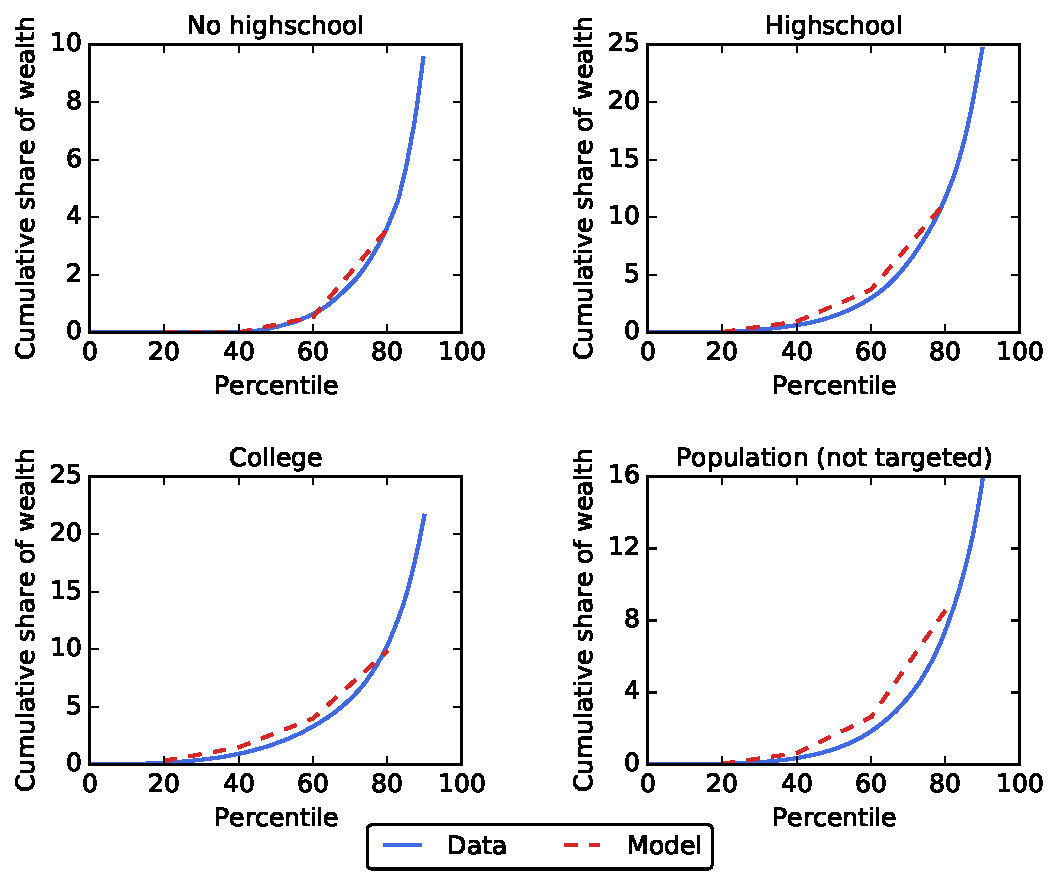
\includegraphics[width=.9\textwidth]{LorenzPoints.pdf}
	\label{fig:LorenzPts}
	\caption{Distributions of liquid wealth within each educational group and for the whole population from the 2004 Survey of Consumer Finance and from the estimated model.}
	\end{center}
\end{figure}

\let\bibfont=\small
\bibliographystyle{econometrica}
\bibliography{Section_calibration_estimation}
%\pdfbookmark[1]{References}{references}

\end{document}